\documentclass[a4paper,12pt]{article} 
\usepackage{graphicx} % Required for inserting images
\usepackage{forest}
\usepackage{tikz}
\usepackage{multicol}
\usepackage{xfrac}
\usetikzlibrary{arrows}

\title{HW3 (Graph Search and MST)}
\author{Isaac Boaz (Solo)}

\begin{document}

\maketitle

\noindent Q1: You are building a computer network for the online beauty product
retailer Glamazon. Glamazon has a number of data centers distributed across the
country (their website is so huge, they need massive compute power) which form a
tree graph. Your job is to pick one special ``hub'' datacenter to host a shared
filesystem for the entire network. The cost of transmitting files across the
network is dominated by the number of links that are traversed, so the hub needs
to be chosen to minimize the number of links. \\
a) Given a tree $T$ containing $n$ nodes, design an efficient algorithm that
computes a hub node $h$. The hub must have the property that the length of the
longest path from $h$ to any other node $v$ is as small as possible. (Hint: Can
leaves ever be hub nodes?) (4 points) \\

The hint of leaves not being hub nodes proves very useful for this problem.
We can analyze this problem from a DP perspective by considering a root problem.
Suppose two nodes, each connected once. Either node may be a hub node, as
the distance from one to the other is 1. If we add a third node, we can see that
the hub node must be the middle node, as the distance from the middle node to
either of the other two nodes is 1; additionally, if we were to make one of the
leaf nodes the hub, we could always pick a better hub by simply moving it to
the center.

This logic can be extended to any tree. We can start by removing all leaf nodes
from the tree, as they can never be hub nodes. We can then remove the new leaf
nodes generated by this, and continue this process until we are left with a
single node.

While sometimes this will leave us with one node left (which is the hub), other
times we will be left with two nodes. In this case, we can simply pick either
node as the hub, as the distance from one to the other is 1.
\\
b) Prove that your algorithm is correct. (4 points) \\
This algorithm can be imagined as simply starting at the hub node that we
picked and removing the furthest leaf nodes recursively. This is guaranteed to
work because the hub node is always the node that is the furthest from any leaf
node.
\\
c) Is the hub unique? How many different hubs can a tree have? (2 points) \\
Since a tree cannot have cycles, a tree can have at most two hubs. If a tree
has two hubs, they must be connected by a single edge, as the distance from one
to the other is 1. \\
\\
Q2: Regarding Depth-First Search: \\
a) Give a counterexample to the conjecture that if a directed graph $G$ contains
a path from $u$ to $v$, and if $u.d < v.d$ in a depth-first search of $G$, then
$v$ is a descendant of $u$ in the depth-first forest produced. (2 points) \\
\\
\begin{multicols}{2}
    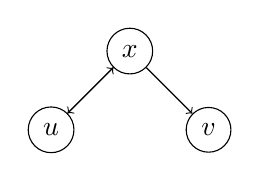
\begin{tikzpicture}
        % Define node styles
        \node [circle, draw, minimum size=1.5em] (u) at (0,0) {$u$};
        \node [circle, draw, minimum size=1.5em] (x) at (1,1) {$x$};
        \node [circle, draw, minimum size=1.5em] (v) at (2,0) {$v$};

        % Draw edges with arrowheads
        \draw [->] (u) -- (x);
        \draw [->] (x) -- (u);
        \draw [->] (x) -- (v);
    \end{tikzpicture}
    \columnbreak
    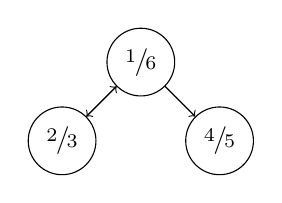
\begin{tikzpicture}
        % Define node styles
        \node [circle, draw, minimum size=1.5em] (u) at (0,0) {$\sfrac{2}{3}$};
        \node [circle, draw, minimum size=1.5em] (x) at (1,1) {$\sfrac{1}{6}$};
        \node [circle, draw, minimum size=1.5em] (v) at (2,0) {$\sfrac{4}{5}$};
        \draw [->] (u) -- (x);
        \draw [->] (x) -- (u);
        \draw [->] (x) -- (v);
    \end{tikzpicture}
\end{multicols}
In this graph if we start at \(x\) and then navigate to \(u\), \(x.d = 1\) and
\(u.d = 2\), further exploring we would get \(v.d = 4\), but in the generated
depth-first forest, \(v\) is not a descendant of \(u\). \\

\begin{forest}
    for tree={circle, draw, minimum size=1.5em, s sep=1em}
    [x
        [u]
        [v]
    ]
\end{forest}
b): Give a counterexample to the conjecture that if a directed graph $G$
contains a path from $u$ to $v$, then any depth-first search must result in $v.d
    \leq u.f$. (2 points)
\\
The above example also serves as a counterexample to this conjecture. In the
depth-first search of the graph, \(v.d = 4\) and \(u.f = 3\), which violates the
conjecture. \\

Q3: Let $G=(V,E)$ be an undirected graph, and let each edge $e \in E$ have
weight $w(e)$. There are 9 vertices in $G,$ all edges have either $w(e)=1$ or
$w(e)=2$, and if you call $E^{'} = \{e \in E:w(e) = 1\},$ you have that
$G'=(V,E')$ is a graph with two connected components. Using this information,
can you determine the weight of a minimum spanning tree in $G$? (6 points)

Regardless of the arrangement of the edges, we would have to pick one single
edge of weight 2 to use to connected the two components. Thus, the total
weight of the minimum spanning tree would be 9.

Since we know removing the \(w(e) = 2\) edges gives us
only 2 connected componenets, we know all \(w(e) = 2\)
edges must then be used to connect the two components.

Thus, we only have to cross one edge of weight 2 to connect the two components,
and the rest of the edges can be of weight 1.
\end{document}

